\documentclass[twoside]{book}

% Packages required by doxygen
\usepackage{fixltx2e}
\usepackage{calc}
\usepackage{doxygen}
\usepackage[export]{adjustbox} % also loads graphicx
\usepackage{graphicx}
\usepackage[utf8]{inputenc}
\usepackage{makeidx}
\usepackage{multicol}
\usepackage{multirow}
\PassOptionsToPackage{warn}{textcomp}
\usepackage{textcomp}
\usepackage[nointegrals]{wasysym}
\usepackage[table]{xcolor}

% Font selection
\usepackage[T1]{fontenc}
\usepackage[scaled=.90]{helvet}
\usepackage{courier}
\usepackage{amssymb}
\usepackage{sectsty}
\renewcommand{\familydefault}{\sfdefault}
\allsectionsfont{%
  \fontseries{bc}\selectfont%
  \color{darkgray}%
}
\renewcommand{\DoxyLabelFont}{%
  \fontseries{bc}\selectfont%
  \color{darkgray}%
}
\newcommand{\+}{\discretionary{\mbox{\scriptsize$\hookleftarrow$}}{}{}}

% Page & text layout
\usepackage{geometry}
\geometry{%
  a4paper,%
  top=2.5cm,%
  bottom=2.5cm,%
  left=2.5cm,%
  right=2.5cm%
}
\tolerance=750
\hfuzz=15pt
\hbadness=750
\setlength{\emergencystretch}{15pt}
\setlength{\parindent}{0cm}
\setlength{\parskip}{3ex plus 2ex minus 2ex}
\makeatletter
\renewcommand{\paragraph}{%
  \@startsection{paragraph}{4}{0ex}{-1.0ex}{1.0ex}{%
    \normalfont\normalsize\bfseries\SS@parafont%
  }%
}
\renewcommand{\subparagraph}{%
  \@startsection{subparagraph}{5}{0ex}{-1.0ex}{1.0ex}{%
    \normalfont\normalsize\bfseries\SS@subparafont%
  }%
}
\makeatother

% Headers & footers
\usepackage{fancyhdr}
\pagestyle{fancyplain}
\fancyhead[LE]{\fancyplain{}{\bfseries\thepage}}
\fancyhead[CE]{\fancyplain{}{}}
\fancyhead[RE]{\fancyplain{}{\bfseries\leftmark}}
\fancyhead[LO]{\fancyplain{}{\bfseries\rightmark}}
\fancyhead[CO]{\fancyplain{}{}}
\fancyhead[RO]{\fancyplain{}{\bfseries\thepage}}
\fancyfoot[LE]{\fancyplain{}{}}
\fancyfoot[CE]{\fancyplain{}{}}
\fancyfoot[RE]{\fancyplain{}{\bfseries\scriptsize Generated by Doxygen }}
\fancyfoot[LO]{\fancyplain{}{\bfseries\scriptsize Generated by Doxygen }}
\fancyfoot[CO]{\fancyplain{}{}}
\fancyfoot[RO]{\fancyplain{}{}}
\renewcommand{\footrulewidth}{0.4pt}
\renewcommand{\chaptermark}[1]{%
  \markboth{#1}{}%
}
\renewcommand{\sectionmark}[1]{%
  \markright{\thesection\ #1}%
}

% Indices & bibliography
\usepackage{natbib}
\usepackage[titles]{tocloft}
\setcounter{tocdepth}{3}
\setcounter{secnumdepth}{5}
\makeindex

% Hyperlinks (required, but should be loaded last)
\usepackage{ifpdf}
\ifpdf
  \usepackage[pdftex,pagebackref=true]{hyperref}
\else
  \usepackage[ps2pdf,pagebackref=true]{hyperref}
\fi
\hypersetup{%
  colorlinks=true,%
  linkcolor=blue,%
  citecolor=blue,%
  unicode%
}

% Custom commands
\newcommand{\clearemptydoublepage}{%
  \newpage{\pagestyle{empty}\cleardoublepage}%
}

\usepackage{caption}
\captionsetup{labelsep=space,justification=centering,font={bf},singlelinecheck=off,skip=4pt,position=top}

%===== C O N T E N T S =====

\begin{document}

% Titlepage & ToC
\hypersetup{pageanchor=false,
             bookmarksnumbered=true,
             pdfencoding=unicode
            }
\pagenumbering{alph}
\begin{titlepage}
\vspace*{7cm}
\begin{center}%
{\Large My Project }\\
\vspace*{1cm}
{\large Generated by Doxygen 1.8.13}\\
\end{center}
\end{titlepage}
\clearemptydoublepage
\pagenumbering{roman}
\tableofcontents
\clearemptydoublepage
\pagenumbering{arabic}
\hypersetup{pageanchor=true}

%--- Begin generated contents ---
\chapter{Class Index}
\section{Class List}
Here are the classes, structs, unions and interfaces with brief descriptions\+:\begin{DoxyCompactList}
\item\contentsline{section}{\hyperlink{structNoeud}{Noeud} }{\pageref{structNoeud}}{}
\end{DoxyCompactList}

\chapter{File Index}
\section{File List}
Here is a list of all documented files with brief descriptions\+:\begin{DoxyCompactList}
\item\contentsline{section}{\hyperlink{huf_8c}{huf.\+c} \\*Compresseur }{\pageref{huf_8c}}{}
\item\contentsline{section}{{\bfseries huf.\+h} }{\pageref{huf_8h}}{}
\end{DoxyCompactList}

\chapter{Class Documentation}
\hypertarget{structNoeud}{}\section{Noeud Struct Reference}
\label{structNoeud}\index{Noeud@{Noeud}}
\subsection*{Public Attributes}
\begin{DoxyCompactItemize}
\item 
\mbox{\Hypertarget{structNoeud_a67400f9553fd71df5a67cf32dc2ab639}\label{structNoeud_a67400f9553fd71df5a67cf32dc2ab639}} 
int {\bfseries fd}
\item 
\mbox{\Hypertarget{structNoeud_a2aeffae918ba8274b8b5f75706bb84de}\label{structNoeud_a2aeffae918ba8274b8b5f75706bb84de}} 
int {\bfseries fg}
\item 
\mbox{\Hypertarget{structNoeud_a2ea9146a5bd3678a27f8a56c9306de22}\label{structNoeud_a2ea9146a5bd3678a27f8a56c9306de22}} 
int {\bfseries pere}
\item 
\mbox{\Hypertarget{structNoeud_a071a0f516c9cd3bba249663d3dbd9a93}\label{structNoeud_a071a0f516c9cd3bba249663d3dbd9a93}} 
double {\bfseries fr}
\end{DoxyCompactItemize}


The documentation for this struct was generated from the following file\+:\begin{DoxyCompactItemize}
\item 
huf.\+h\end{DoxyCompactItemize}

\chapter{File Documentation}
\hypertarget{huf_8c}{}\section{huf.\+c File Reference}
\label{huf_8c}\index{huf.\+c@{huf.\+c}}


Compresseur.  


{\ttfamily \#include $<$stdlib.\+h$>$}\newline
{\ttfamily \#include $<$stdio.\+h$>$}\newline
{\ttfamily \#include $<$string.\+h$>$}\newline
{\ttfamily \#include \char`\"{}huf.\+h\char`\"{}}\newline
Include dependency graph for huf.\+c\+:
\nopagebreak
\begin{figure}[H]
\begin{center}
\leavevmode
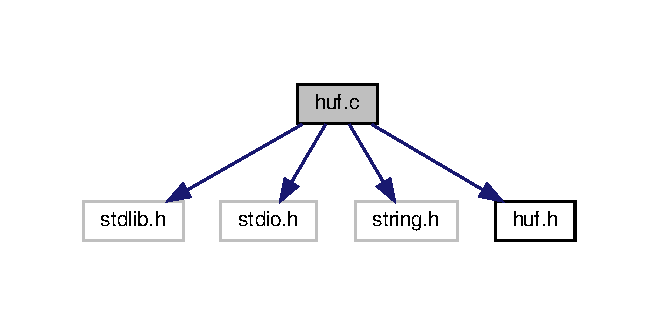
\includegraphics[width=316pt]{huf_8c__incl}
\end{center}
\end{figure}
\subsection*{Functions}
\begin{DoxyCompactItemize}
\item 
\mbox{\Hypertarget{huf_8c_af3a761f4d61ef26e5209b428d977da4f}\label{huf_8c_af3a761f4d61ef26e5209b428d977da4f}} 
void {\bfseries calcul\+Freq} (char $\ast$fichier)
\item 
\mbox{\Hypertarget{huf_8c_a5f279d4f0903b03455ccd8b26a9170c7}\label{huf_8c_a5f279d4f0903b03455ccd8b26a9170c7}} 
void {\bfseries affiche\+Freq} ()
\item 
\mbox{\Hypertarget{huf_8c_a79a3701ceb6a1cc2fa23acdd0e1e5427}\label{huf_8c_a79a3701ceb6a1cc2fa23acdd0e1e5427}} 
void {\bfseries init\+Arbre} ()
\item 
\mbox{\Hypertarget{huf_8c_ae10b899b8a3196bbc2f5fdb95856dd97}\label{huf_8c_ae10b899b8a3196bbc2f5fdb95856dd97}} 
void {\bfseries affiche\+Arbre} ()
\item 
\mbox{\Hypertarget{huf_8c_a7c1e4d5f951b5b24771c5b000a8d94d7}\label{huf_8c_a7c1e4d5f951b5b24771c5b000a8d94d7}} 
void {\bfseries construct\+Arbre} ()
\item 
\mbox{\Hypertarget{huf_8c_a8fee947ba260b5049ea5b33048b0cf63}\label{huf_8c_a8fee947ba260b5049ea5b33048b0cf63}} 
void {\bfseries parcours} (int indice\+Noeud, char $\ast$code)
\item 
\mbox{\Hypertarget{huf_8c_ade9ffb32e10a0cc2be0c4ac98b39f96f}\label{huf_8c_ade9ffb32e10a0cc2be0c4ac98b39f96f}} 
void {\bfseries del\+\_\+char} (char $\ast$str, char c)
\item 
\mbox{\Hypertarget{huf_8c_a5dfef645b3ad6843612c13686a4d1222}\label{huf_8c_a5dfef645b3ad6843612c13686a4d1222}} 
void {\bfseries cree\+Fiche} (char $\ast$fichier)
\item 
\mbox{\Hypertarget{huf_8c_a3c04138a5bfe5d72780bb7e82a18e627}\label{huf_8c_a3c04138a5bfe5d72780bb7e82a18e627}} 
int {\bfseries main} (int argc, char $\ast$$\ast$argv)
\end{DoxyCompactItemize}


\subsection{Detailed Description}
Compresseur. 

\begin{DoxyAuthor}{Author}
Ambre.\+Lamouchi Alexandre.\+Canton.\+Condes 
\end{DoxyAuthor}
\begin{DoxyVersion}{Version}
1.\+0 
\end{DoxyVersion}
\begin{DoxyDate}{Date}
7 décembre 2018
\end{DoxyDate}
Programme de compression utilisant l\textquotesingle{}algorithme de Huffman 
%--- End generated contents ---

% Index
\backmatter
\newpage
\phantomsection
\clearemptydoublepage
\addcontentsline{toc}{chapter}{Index}
\printindex

\end{document}
